% Terminology-aware distillation for vocational content (IEEE conference format).
% Build:  tectonic -X compile main.tex   (XeLaTeX engine; Devanagari via fontspec)
\documentclass[conference]{IEEEtran}

\usepackage{fontspec}
\setmainfont{texgyretermes}[Extension=.otf,UprightFont=*-regular,BoldFont=*-bold,ItalicFont=*-italic,BoldItalicFont=*-bolditalic]
\newfontfamily\devfont{NotoSansDevanagariUI}[Path=fonts/,Extension=.ttf,UprightFont=*-Regular,BoldFont=*-Bold,Script=Devanagari,Scale=0.92]
\newcommand{\dev}[1]{{\devfont #1}}

\usepackage{amsmath,amssymb}
\usepackage{cite}
\usepackage{graphicx}
\usepackage{booktabs}
\usepackage{multirow}
\usepackage{array}
\usepackage{xcolor}
\usepackage{tikz}
\usetikzlibrary{arrows.meta,positioning,fit,calc}
\usepackage{url}

\newcommand{\sig}{$^{\uparrow}$}   % significant gain over base (p < 0.05)
\newcommand{\sigd}{$^{\downarrow}$} % significant loss vs base (p > 0.95)

\begin{document}

\title{Terminology-Aware Knowledge Distillation for Translating Vocational Electrician Training Content into Low-Resource Indian Languages}

\author{\IEEEauthorblockN{Gaurav}
\IEEEauthorblockA{AIT-CSE, Chandigarh University\\
Mohali-140413, Punjab, India\\
gauravgoswami967@gmail.com}
\and
\IEEEauthorblockN{Aastha Shukla}
\IEEEauthorblockA{AIT-CSE, Chandigarh University\\
Mohali-140413, Punjab, India\\
aasthashukla360@gmail.com}
\and
\IEEEauthorblockN{Anubhav Sharma}
\IEEEauthorblockA{AIT-CSE, Chandigarh University\\
Mohali-140413, Punjab, India\\
anubhavsharma1049@gmail.com}}

\maketitle

\begin{abstract}
Vocational training material in India is written mostly in English, while many trainees learn better in their own language. Technical terms are the hardest part of translating this material, and a wrong term in an electrical safety instruction can mislead a trainee. We study English-to-Indic translation of electrician training content for Hindi and three low-resource languages, Konkani, Maithili and Dogri, in a formal technical register based on standard Hindi terminology. We extract 24,636 English sentences from nine official electrician books and distill IndicTrans2-1B into the 200M-parameter IndicTrans2 model with low-rank adaptation. The teacher rarely uses the formal terms and often chooses words with the wrong meaning: in three of the four languages it translates \emph{three phase} with the word for ``stage'' in 94--100\% of sentences, and plain distillation passes these choices to the student. We therefore repair the teacher's translations before training. Each glossary term is replaced by an entity placeholder that the teacher copies into place, the formal term is inserted afterwards, and detached case endings are re-attached. The resulting student reaches 90--99.6\% formal-term compliance averaged over term types, against 28--51\% for the base model, with no measurable loss on the IN22-Gen benchmark. Constrained decoding and placeholders at inference time give similar compliance but cost 0.9--9.3 chrF++ points against the teacher's translations, while a hybrid fallback that re-translates only sentences with a missing term reaches 100\% at a mean cost of 0.3 points.
\end{abstract}

\begin{IEEEkeywords}
machine translation, terminology, knowledge distillation, low-resource languages, Indian languages, vocational education, parameter-efficient fine-tuning
\end{IEEEkeywords}

% ============================================================================
\section{Introduction}

India trains electricians, fitters and other tradespeople through Industrial Training Institutes under the Directorate General of Training. The trade books used in these courses are published mainly in English, and trainees from many regions read them in a second or third language. Machine translation (MT) could produce local-language editions at low cost, and open models now cover all 22 scheduled languages of India~\cite{gala2023indictrans2}. Electrical training text, however, depends on a small set of technical terms, and these terms carry safety meaning. A translation that renders \emph{three phase} as ``three stages'' or \emph{earthing} as ``the planet Earth'' reads fluently and still teaches the wrong concept.

A second difficulty is register. Hindi technical writing can use English loanwords written in Devanagari (\dev{वोल्टेज}, \dev{अर्थिंग}) or standardized native terms of the kind found in school textbooks and government glossaries (\dev{वोल्टता}, \dev{भूसंपर्कन})~\cite{ncert_science10,cstt}. Educational material needs one register applied consistently. In this work we target the formal register and treat the choice as a design parameter: the same method applies to a loanword glossary.

Parallel data for this domain does not exist. We found no official Indian-language edition of the electrician books, so we build training data by forward translation with a strong teacher model and distill it into a smaller student~\cite{kim2016sequence}. We study what happens to terminology when a student learns from a teacher's output. The teacher's terminology habits, including wrong-sense renderings, transfer to the student almost unchanged, and they can be corrected in the training data before distillation.

Our contributions are:
\begin{itemize}
\item A corpus of 24,636 English sentences from nine official electrician trade books with a split by page blocks that prevents near-duplicate leakage, and a two-register glossary of 32 terms for Hindi, Konkani, Maithili and Dogri.
\item An analysis showing that IndicTrans2-1B uses the formal term in only 32--40\% of term-bearing sentences and produces wrong-sense terms systematically, and that plain sequence-level distillation inherits this behaviour (Konkani macro compliance falls from 27.9\% to 20.2\%).
\item Terminology-aware distillation: an offline repair of the teacher's translations that reuses the teacher's own entity-placeholder mechanism, followed by validation and re-attachment of case endings. The repaired student reaches 90--99.6\% macro compliance without inference-time constraints and keeps its general-domain quality.
\item A comparison with inference-time enforcement (constrained decoding, placeholders, and a hybrid fallback), and an analysis of seed variance, joint versus single-language training, and the effect of placeholders on morphology.
\end{itemize}

% ============================================================================
\section{Related Work}

\subsection{Machine Translation for Indian Languages}
Large parallel corpora such as Samanantar~\cite{ramesh2022samanantar} and monolingual resources such as IndicNLPSuite~\cite{kakwani2020indicnlpsuite} enabled strong Indic MT systems. IndicTrans2~\cite{gala2023indictrans2} provides Transformer~\cite{vaswani2017attention} models for all 22 scheduled languages, trained on the BPCC corpus and evaluated on the IN22 benchmark, in a 1B-parameter version and distilled 200M versions; it covers all four of our target languages, and the two model sizes suit a teacher--student setup. NLLB-200~\cite{nllb2022} extends a single model to 200 languages. Both follow the tagged multilingual design~\cite{johnson2017google,dabre2020survey}, are trained mostly on general-domain data, and are not tuned to any technical register.

\subsection{Domain Adaptation and Parameter-Efficient Fine-Tuning}
Domain mismatch is a known weakness of neural MT~\cite{koehn2017six}, and continued training on in-domain data is the standard remedy~\cite{luong2015stanford,freitag2016fast,chu2018survey,saunders2022domain}. Full fine-tuning can degrade general-domain quality (catastrophic forgetting), which motivates regularized training~\cite{thompson2019overcoming}. Adapter modules~\cite{houlsby2019parameter,bapna2019simple} and low-rank adaptation (LoRA)~\cite{hu2022lora} train a small number of added parameters while the base model stays fixed, which limits forgetting and keeps per-domain artifacts small. We use LoRA and measure forgetting on IN22-Gen.

\subsection{Distillation and Synthetic Parallel Data}
Sequence-level knowledge distillation trains a student on the teacher's beam-search output~\cite{kim2016sequence}. When only source-side text exists, forward translation of in-domain monolingual data is a related form of self-training~\cite{zhang2016exploiting}, complementary to back-translation of target-side text~\cite{sennrich2016improving}. Work in this line usually measures overall quality. We look at a specific property, terminology, and show that the teacher's systematic term choices pass into the student.

\subsection{Terminology in Neural MT}
Lexically constrained decoding forces given target phrases into the output, using grid beam search~\cite{hokamp2017lexically}, dynamic beam allocation~\cite{post2018fast,hu2019improved} or finite-state constraints~\cite{hasler2018neural}. These methods guarantee that a phrase appears but can harm fluency and slow decoding. Training-time methods instead teach a model to follow terminology hints, by inline annotation of target terms in the source~\cite{dinu2019training} or by code-switching source terms with their translations~\cite{song2019code}. Placeholder tokens that the model copies through translation were used for rare words~\cite{luong2015addressing} and named entities~\cite{crego2016systran}. The WMT 2023 shared task on terminology~\cite{semenov2023findings} evaluated several of these approaches. Our method differs in where the terminology enters: we change the distillation data offline, using the teacher's own placeholder handling, so the student needs no special input format or decoding procedure. We also study a register-level glossary rather than isolated term pairs, in morphologically rich low-resource languages.

% ============================================================================
\section{Problem Formulation}

Let $\ell$ be a target language and $\mathcal{G}_\ell$ a glossary that maps each English term $e$ to a set $F_\ell(e)$ of accepted target forms (the formal term and its spelling variants). For a source sentence $x$, let $T(x)$ be the glossary terms that occur in $x$, and let $\hat{y}$ be a system output. A normalization function $\nu$ maps spelling variants of the same word to one form (Section~\ref{sec:metrics}). We say $\hat{y}$ \emph{uses} $e$ if some $f \in F_\ell(e)$ satisfies $\nu(f) \sqsubseteq \nu(\hat{y})$, where $\sqsubseteq$ denotes substring occurrence. Pooled term compliance over a test set $D$ is
\begin{equation}
C_{\text{pool}} = \frac{\sum_{x \in D} \sum_{e \in T(x)} \mathbb{1}\left[\hat{y}_x \text{ uses } e\right]}{\sum_{x \in D} |T(x)|}.
\end{equation}
Because a few terms can dominate $D$, we also report macro compliance, the mean of per-term compliance over the set $E$ of term types in $D$:
\begin{equation}
C_{\text{macro}} = \frac{1}{|E|} \sum_{e \in E} \frac{\sum_{x: e \in T(x)} \mathbb{1}\left[\hat{y}_x \text{ uses } e\right]}{|\{x : e \in T(x)\}|}.
\end{equation}
Compliance does not need a reference translation. It measures adherence to the chosen register, and a correct loanword counts as non-compliant.

We distinguish two kinds of non-compliance. A \emph{register mismatch} uses a correct concept in the other register (\dev{वोल्टेज} for \dev{वोल्टता}). A \emph{wrong-sense rendering} uses a word with a different meaning, such as \dev{चरण} (``stage, step'') for electrical phase or \dev{पृथ्वी} (``the planet Earth'') for earthing. Both break consistency; the second also misinforms the reader.

We ask three research questions. RQ1: How well do the teacher and the base student follow a formal glossary, and does sequence-level distillation change this? RQ2: Can terminology be corrected in the distillation data so that the student follows the glossary without inference-time constraints, and at what cost in general quality? RQ3: How does this compare with enforcing terminology at inference time?

% ============================================================================
\section{Data and Resources}
\label{sec:data}

\subsection{Source Corpus}
We use nine Electrician trade books published by the National Instructional Media Institute for the Directorate General of Training~\cite{nimi_electrician}: Trade Theory and Trade Practical for the Craft Instructor Training Scheme, Trade Theory for semesters 1--4 and Trade Practical for semesters 2 and 4 of the Craftsmen Training Scheme, and one question paper (2,143 pages in total). Text is extracted page by page with PyMuPDF~\cite{pymupdf}. We remove running headers and footers (lines found on at least 5\% of pages), rejoin wrapped lines and hyphenated breaks, and split sentences by rule. We keep sentences of 5--45 words that start with a capital, end with punctuation, are mostly letters (at least 60\% letters, at most 20\% digits and 50\% capitals) and contain no URL or publisher notice, and remove exact duplicates (Table~\ref{tab:corpus}).

\begin{table}[t]
\caption{Corpus statistics. The split is made by blocks of ten consecutive pages.}
\label{tab:corpus}
\centering
\footnotesize
\begin{tabular}{@{}lr@{}}
\toprule
Source books / pages & 9 / 2,143 \\
English sentences (filtered, all splits) & 24,636 \\
Train / dev / test sentences & 24,082 / 354 / 200 \\
Test sentences with a domain term & 150 \\
Glossary-term occurrences in test (per language) & 140 (15 types) \\
Occurrences of the most frequent term (\emph{conduit}) & 65 (46\%) \\
\bottomrule
\end{tabular}
\end{table}

To prevent leakage, the split assigns whole blocks of ten consecutive pages to the test, dev and training sets, with a fixed seed. From the test blocks we select 200 sentences, 75\% of them containing domain terms; the remaining test-block sentences are discarded rather than moved to training. Training sentences whose word 4-gram Jaccard similarity to any dev or test sentence is at least 0.7 are also removed. Because one test block comes from a chapter on conduit wiring, \emph{conduit} accounts for 46\% of test-set term occurrences, which is why we report macro compliance.

\subsection{Glossary}
The glossary has 32 English terms that are frequent in the books (for example \emph{voltage}, \emph{earthing}, \emph{three phase}, \emph{circuit breaker}, \emph{megger}) with two registers per language: a formal register and a loanword register for comparison. Each formal entry has a status: \emph{standard} (an established term in NCERT science textbooks or CSTT usage~\cite{ncert_science10,cstt}; 11 Hindi entries), \emph{proposed} (author-curated), or \emph{loanword kept} where no native term is in common use (cable, fuse, megger, main switch, terminal block). The Konkani, Maithili and Dogri entries follow the Hindi technical register with the grammar and spelling of each language, for example Dogri \dev{मुक्ख} for ``main''. Table~\ref{tab:glossary} shows Hindi examples. The glossary was not reviewed by native-speaker instructors; we discuss this limitation in Section~\ref{sec:limitations}.

\begin{table}[t]
\caption{Hindi glossary examples: loanword register, formal register, and the teacher's usual rendering in the training/dev drafts.}
\label{tab:glossary}
\centering
\footnotesize
\setlength{\tabcolsep}{3pt}
\begin{tabular}{@{}llll@{}}
\toprule
English & Loanword & Formal & Teacher (usual) \\
\midrule
three phase & \dev{थ्री फेज} & \dev{त्रिकला} & \dev{तीन चरण} (``three stages'') \\
earthing & \dev{अर्थिंग} & \dev{भूसंपर्कन} & \dev{अर्थिंग}; \dev{पृथ्वी} (``Earth'') \\
live wire & \dev{लाइव तार} & \dev{विद्युन्मय तार} & \dev{जीवित तार} (``living wire'') \\
insulation & \dev{इन्सुलेशन} & \dev{विद्युतरोधन} & \dev{इन्सुलेशन} \\
voltage & \dev{वोल्टेज} & \dev{वोल्टता} & \dev{वोल्टेज} \\
circuit breaker & \dev{सर्किट ब्रेकर} & \dev{परिपथ वियोजक} & \dev{सर्किट ब्रेकर} \\
megger & \dev{मेगर} & \dev{मेगर} (kept) & \dev{मेगर} \\
\bottomrule
\end{tabular}
\end{table}

\subsection{Benchmark}
General-domain quality is measured on IN22-Gen~\cite{gala2023indictrans2}, 1,024 sentences with human translations into all 22 scheduled languages. We use it for a reference table of the base model and to test the adapted models for forgetting.

% ============================================================================
\section{Methodology}
\label{sec:method}

\begin{figure*}[t]
\centering
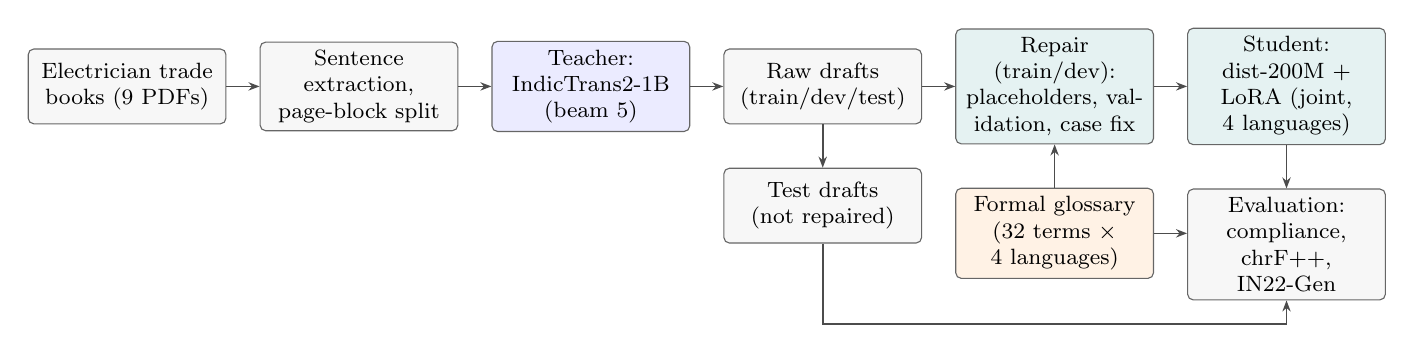
\begin{tikzpicture}[
  font=\footnotesize,
  box/.style={draw=black!60, rounded corners=2pt, fill=#1, align=center, minimum height=0.95cm, inner sep=3pt, text width=2.3cm},
  box/.default=black!3,
  arr/.style={-{Stealth[length=4pt]}, black!70, line width=0.6pt}
]
\node[box] (pdf) {Electrician trade books (9 PDFs)};
\node[box, right=0.42cm of pdf] (sent) {Sentence extraction, page-block split};
\node[box=blue!8, right=0.42cm of sent] (teach) {Teacher: \mbox{IndicTrans2-1B} (beam 5)};
\node[box, right=0.42cm of teach] (raw) {Raw drafts (train/dev/test)};
\node[box=teal!10, right=0.42cm of raw] (rep) {Repair (train/dev): placeholders, validation, case fix};
\node[box=teal!10, right=0.42cm of rep] (stud) {Student: dist-200M + LoRA (joint, 4 languages)};
\node[box=orange!10, below=0.55cm of rep] (gl) {Formal glossary (32 terms $\times$ 4 languages)};
\node[box, below=0.55cm of stud] (eval) {Evaluation: compliance, chrF++, IN22-Gen};
\node[box, below=0.55cm of raw] (test) {Test drafts (not repaired)};
\draw[arr] (pdf) -- (sent);
\draw[arr] (sent) -- (teach);
\draw[arr] (teach) -- (raw);
\draw[arr] (raw) -- (rep);
\draw[arr] (rep) -- (stud);
\draw[arr] (gl) -- (rep);
\draw[arr] (raw) -- (test);
\draw[arr] (test.south) |- ($(eval.south)+(0,-0.3)$) -- (eval.south);
\draw[arr] (stud) -- (eval);
\draw[arr] (gl.east) -- (gl.east -| eval.west);
\end{tikzpicture}
\caption{Terminology-aware distillation. The teacher translates the in-domain English sentences; training and dev drafts are repaired with the glossary before the student is trained. Test drafts are kept unrepaired so that reference-based scores are not biased toward the method.}
\label{fig:pipeline}
\end{figure*}

\subsection{Teacher--Student Distillation}
Fig.~\ref{fig:pipeline} shows the pipeline. The teacher, IndicTrans2-1B, translates all 24,636 sentences into each target language with beam size 5, after the standard IndicTrans2 preprocessing~\cite{indictranstoolkit}. Batches are sorted by length and capped by a token budget (sentences $\times$ source tokens $\times$ beams $\le$ 8,000), and generation length is capped at twice the source length plus 16 tokens to stop runaway outputs. On one NVIDIA T4 GPU the teacher translates 13--14 sentences per second, about 30 minutes per language. The student is the distilled IndicTrans2 model with 200M parameters.

\subsection{Terminology-Aware Repair}
A training draft needs repair if its source contains a glossary term and the draft does not use an accepted formal form for it. This holds for 3,476--3,869 drafts per language (14--16\% of the corpus). For each such sentence we re-translate the source with the teacher after replacing every English glossary term with an entity placeholder of the form \texttt{<IDn>}. The IndicTrans2 preprocessor already uses such placeholders for URLs, e-mail addresses and some numerals, and the model copies them to the corresponding position in the output. Our placeholder numbers continue after any placeholders created by the preprocessor, so the two never collide. After decoding we replace each placeholder with the formal term, accepting the bracket and Devanagari spellings of ``ID'' that the model sometimes produces.

A repaired draft is rejected if a glossary term is still missing, if a term appears only after the final sentence punctuation, or if its length differs from the original draft by more than a factor of 0.7--1.5. Rejected sentences are dropped from training; test drafts are never repaired. Table~\ref{tab:repair} reports the outcome.

\begin{table}[t]
\caption{Placeholder repair of the training and dev drafts (one T4 GPU).}
\label{tab:repair}
\centering
\footnotesize
\begin{tabular}{@{}lrrrr@{}}
\toprule
 & Hindi & Konkani & Maithili & Dogri \\
\midrule
Drafts needing repair & 3,557 & 3,869 & 3,476 & 3,725 \\
Repaired (\%) & 98.2 & 98.9 & 98.7 & 98.7 \\
Rejected: term still missing & 53 & 23 & 23 & 30 \\
Rejected: length ratio & 7 & 18 & 20 & 15 \\
Rejected: term after sentence end & 3 & 1 & 2 & 3 \\
Time (min) & 6.7 & 7.1 & 5.9 & 6.9 \\
\bottomrule
\end{tabular}
\end{table}

\emph{Case endings.} In Maithili and Konkani several case markers attach to the noun (Maithili \dev{-क}, \dev{-केँ}, \dev{-सँ}; Konkani \dev{-च्या}, \dev{-ची}). With a placeholder in the input, the teacher writes these markers as separate words, so the restored term is followed by a detached ending (\dev{विद्युतरोधन केँ} instead of \dev{विद्युतरोधनकेँ}). In the repaired Maithili drafts, detached endings after glossary terms outnumbered attached ones by 1,211 to 100, while unrepaired drafts showed the reverse (17 to 1,269). We re-attach these markers by rule when they directly follow a glossary term; this changed 1,050 Maithili and 427 Konkani repaired drafts. Hindi and Dogri write postpositions as separate words and need no correction.

\emph{A rejected alternative.} We first tried lexically constrained beam search with disjunctive constraints over each term and its variants. On a 20-sentence pilot with the teacher, only 5 outputs passed validation; in the other 15 the forced term was appended after the sentence, and decoding took about 1.5 seconds per sentence, more than ten times slower than the placeholder method.

\subsection{Student Fine-Tuning}
We train one LoRA adapter jointly on all four languages, with the target language given by the IndicTrans2 language tag. Table~\ref{tab:hyper} lists the settings. Training pairs whose target exceeds 160 tokens or three times the source length are dropped (13--31 per language). The checkpoint with the best dev chrF++ is kept, and only the adapter (26 MB) is saved. We train three models: on the raw drafts (\emph{raw}), on the repaired drafts before the case-ending fix (\emph{r5}), and on the final repaired drafts (\emph{r6}, two seeds).

\begin{table}[t]
\caption{Student fine-tuning settings.}
\label{tab:hyper}
\centering
\footnotesize
\begin{tabular}{@{}ll@{}}
\toprule
Base model & IndicTrans2 en-indic dist-200M \\
Adapter & LoRA, $r=16$, $\alpha=32$, dropout 0.1 \\
Target modules & q, k, v, output projections; FFN layers \\
Trainable parameters & 6.49M of 218.3M (2.97\%) \\
Optimizer & AdamW~\cite{loshchilov2019decoupled}, lr $3\times10^{-4}$, $\beta_2=0.98$ \\
Schedule & inverse square root, 300 warm-up steps \\
Batch & 16 $\times$ 4 accumulation = 64 pairs \\
Regularization & label smoothing 0.1~\cite{szegedy2016rethinking}, weight decay 0.01 \\
Training & 3 epochs (about 4,500 steps), fp16 \\
Model selection & dev chrF++ every 500 steps (800 sent.), patience 4 \\
Training pairs & 96,074 (repaired), 96,248 (raw) \\
Hardware / time & one NVIDIA T4, about 2 hours per model \\
\bottomrule
\end{tabular}
\end{table}

\subsection{Inference-Time Enforcement}
We compare the trained models with three ways of enforcing the glossary at inference time: (i) \emph{placeholders}, which apply the repair procedure above to every term in the test source; (ii) \emph{constrained decoding} with disjunctive lexical constraints; and (iii) a \emph{hybrid} mode that translates normally and re-translates with placeholders only the sentences whose output misses a glossary term, keeping the retry if it reduces the number of missing terms. The hybrid mode also applies the case-ending rule.

% ============================================================================
\section{Experimental Setup}
\label{sec:setup}

\subsection{Systems}
We evaluate the base student (\emph{base}), the student distilled on raw drafts (\emph{raw}), the terminology-aware students (\emph{r5} and \emph{r6}; r6 with seeds 42 and 43), the teacher, and the inference-time variants of base and r5/r6. All systems decode with beam size 5. Training and evaluation ran on Kaggle (NVIDIA T4 GPUs) with Transformers 4.46~\cite{wolf2020transformers}, PEFT 0.13~\cite{peft} and sacreBLEU 2.4, using about 17 GPU-hours in total.

\subsection{Metrics}
\label{sec:metrics}
Term compliance is computed as defined above. The normalization $\nu$ applies Unicode NFC, removes the nukta, maps chandrabindu to anusvara and a nasal consonant with virama before another consonant to anusvara (\dev{इन्सुलेशन} and \dev{इंसुलेशन} become identical), and treats hyphens as spaces. Without it, string matching undercounted teacher compliance by up to 8 points for Dogri. BLEU~\cite{papineni2002bleu} and chrF++~\cite{popovic2015chrf,popovic2017chrf} (character order 6, word order 2) are computed at corpus level with sacreBLEU~\cite{post2018call}. Differences in chrF++ against the base model are tested with paired bootstrap resampling~\cite{koehn2004statistical} (1,000 samples).

\subsection{What the References Measure}
The domain test references are the teacher's translations of the 200 test sentences, produced for post-editing by native speakers, which has not yet been done. Scores against them measure agreement with the teacher, which mostly uses loanwords. They penalize correct formal terms and favour systems that imitate the teacher; even post-edited references would keep part of this bias~\cite{toral2019post}. We therefore read them only as closeness to a strong system and base terminology claims on compliance, which needs no reference. General-domain quality is measured on IN22-Gen, which has human references.

% ============================================================================
\section{Results}

\subsection{Teacher Terminology (RQ1)}
Over training and dev drafts that contain a glossary term, the teacher uses the formal term in 38.8\% (Hindi), 32.0\% (Konkani), 40.0\% (Maithili) and 35.5\% (Dogri) of cases. Against the loanword glossary the same drafts score 83.5--87.4\%, so the teacher's default register is mostly the loanword one. Fig.~\ref{fig:teacher} breaks this down by term. Frequent loanword-register terms such as \emph{voltage}, \emph{voltmeter} and \emph{circuit breaker} receive no formal renderings at all, while \emph{resistance} agrees with the formal glossary, as do \emph{fuse} and \emph{megger}, whose loanwords serve as the formal form. Table~\ref{tab:wrongsense} counts wrong-sense renderings. The Hindi word \dev{चरण} (``stage'') appears for \emph{three phase} in 94--100\% of Hindi, Maithili and Dogri drafts, and \dev{जीवित}/\dev{जींदे} (``living'') appears in 56--81\% of drafts containing \emph{live wire}.

\begin{figure}[t]
\centering
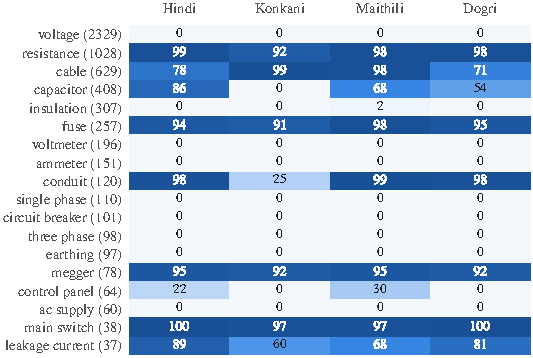
\includegraphics[width=\columnwidth]{figures/fig_teacher_consistency.pdf}
\caption{Share (\%) of teacher training/dev drafts that use the formal glossary term, for terms with at least 30 sentences (count in parentheses).}
\label{fig:teacher}
\end{figure}

\begin{table}[t]
\caption{Wrong-sense renderings in the teacher's training/dev drafts: share of drafts containing the English term whose translation contains the wrong-sense word.}
\label{tab:wrongsense}
\centering
\footnotesize
\setlength{\tabcolsep}{4pt}
\begin{tabular}{@{}llrrrr@{}}
\toprule
Term (n) & Wrong-sense word & Hindi & Konk. & Maith. & Dogri \\
\midrule
three phase (98) & \dev{चरण} ``stage'' & 95.9 & 0.0 & 93.9 & 100.0 \\
single phase (110) & \dev{चरण} ``stage'' & 93.6 & 0.0 & 96.4 & 82.7 \\
live wire (16) & ``living'' & 81.2 & 56.2 & 68.8 & 62.5 \\
earthing (97) & ``earth, soil'' & 59.8 & 40.2 & 38.1 & 73.2 \\
\bottomrule
\end{tabular}
\end{table}

\subsection{Term Compliance After Distillation (RQ1, RQ2)}
Table~\ref{tab:main} and Fig.~\ref{fig:compliance} give the main results. The base student and the teacher reach 28--51\% macro compliance. Distillation on raw drafts does not improve this and lowers it in three languages; for Konkani macro compliance falls from 27.9\% to 20.2\% and pooled compliance from 39.3\% to 20.7\%, because the student adopts the teacher's loanwords. The terminology-aware students reach 90.0--99.6\% macro compliance (r6, seed 42) and 97.0--99.3\% pooled compliance. The two seeds agree within 3.3 points of macro compliance. Excluding the dominant term \emph{conduit} does not change the picture: pooled compliance without it is 25.3--37.3\% for base and 93.3--98.7\% for r6.

\begin{table*}[t]
\caption{Domain test set (200 sentences per language). Comp.\ = formal-term compliance (\%), pooled / macro. chrF++ and BLEU are measured against the teacher's unedited translations and indicate agreement with the teacher, not human-judged quality. \sig/\sigd: significantly higher/lower chrF++ than base (paired bootstrap, $p<0.05$).}
\label{tab:main}
\centering
\footnotesize
\setlength{\tabcolsep}{3.2pt}
\begin{tabular}{@{}l ccc ccc ccc ccc@{}}
\toprule
 & \multicolumn{3}{c}{Hindi} & \multicolumn{3}{c}{Konkani} & \multicolumn{3}{c}{Maithili} & \multicolumn{3}{c}{Dogri} \\
\cmidrule(lr){2-4}\cmidrule(lr){5-7}\cmidrule(lr){8-10}\cmidrule(l){11-13}
System & Comp. & chrF++ & BLEU & Comp. & chrF++ & BLEU & Comp. & chrF++ & BLEU & Comp. & chrF++ & BLEU \\
\midrule
Base (dist-200M) & 61.4 / 43.4 & 86.6 & 78.0 & 39.3 / 27.9 & 70.8 & 51.5 & 64.3 / 50.8 & 74.1 & 55.8 & 55.7 / 32.1 & 75.6 & 61.1 \\
Distilled, raw drafts & 62.1 / 36.4 & 87.4 & 79.0 & 20.7 / 20.2 & 76.9\sig & 60.8 & 63.6 / 43.5 & 77.2\sig & 59.6 & 59.3 / 31.7 & 82.6\sig & 71.8 \\
Term-aware r5 & 98.6 / 93.3 & 84.2\sigd & 75.7 & 95.7 / 97.6 & 72.8\sig & 56.1 & 98.6 / 99.5 & 75.2 & 57.4 & 98.6 / 93.3 & 79.2\sig & 68.7 \\
Term-aware r6, seed 42 & 98.6 / 93.3 & 83.8\sigd & 74.8 & 95.0 / 97.6 & 72.4 & 55.7 & 99.3 / 99.6 & 74.4 & 55.2 & 97.9 / 90.0 & 79.3\sig & 68.9 \\
Term-aware r6, seed 43 & 98.6 / 93.3 & 83.9\sigd & 74.9 & 91.4 / 96.0 & 73.4\sig & 56.8 & 99.3 / 99.6 & 74.1 & 56.1 & 98.6 / 93.3 & 79.3\sig & 68.7 \\
r6 + hybrid fallback & 100 / 100 & 83.6\sigd & 74.6 & 100 / 100 & 71.6 & 54.9 & 100 / 100 & 74.2 & 55.1 & 100 / 100 & 79.1\sig & 68.6 \\
\midrule
Teacher (1B) & 62.9 / 42.4 & -- & -- & 25.0 / 20.1 & -- & -- & 64.3 / 46.8 & -- & -- & 55.7 / 32.9 & -- & -- \\
\bottomrule
\end{tabular}
\end{table*}

\begin{figure}[t]
\centering
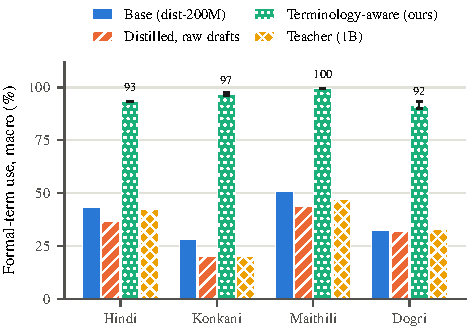
\includegraphics[width=\columnwidth]{figures/fig_compliance.pdf}
\caption{Macro formal-term compliance on the test set. For the terminology-aware model (r6) the bar is the mean of two seeds and the whisker spans both.}
\label{fig:compliance}
\end{figure}

Against the teacher's translations, the raw-draft student is the closest to the teacher, as expected for a model trained to imitate it, with significant chrF++ gains over base for Konkani, Maithili and Dogri. The terminology-aware students score lower than the raw-draft student on this measure because every formal term they produce differs from the teacher's loanword. They still exceed base significantly for Dogri (+3.7 chrF++) and nearly so for Konkani (+1.6, $p=0.052$), and are 2.8 points below base for Hindi, where the base model is already close to the teacher. We do not read these differences as quality differences, for the reason given in Section~\ref{sec:setup}.

The examples in Table~\ref{tab:examples} show typical changes. The base model and the raw-draft student write \dev{एकल चरण} for \emph{single phase}; the terminology-aware student writes \dev{एकल कला}. In Hindi, Maithili and Dogri, base and raw-draft outputs contain \dev{चरण} in both \emph{single phase} test sentences, and r6 outputs in neither. The student also inflects formal terms by itself (\dev{परिपथ वियोजकों}, plural oblique), which an inference-time substitution cannot do.

\begin{table}[t]
\caption{Test-set examples (excerpts). Glossary terms in bold.}
\label{tab:examples}
\centering
\footnotesize
\setlength{\tabcolsep}{3pt}
\begin{tabular}{@{}p{0.11\columnwidth}p{0.83\columnwidth}@{}}
\toprule
\multicolumn{2}{@{}p{0.96\columnwidth}}{\emph{\dots\ service line pole for \textbf{single phase} 230 V distribution\dots} (Hindi)} \\
Base & \dev{खुले स्थान में \textbf{एकल चरण} 230 वी वितरण प्रणाली के लिए…} \\
Raw & \dev{खुले स्थान में \textbf{एकल चरण} 230 वी वितरण प्रणाली के लिए…} \\
r6 & \dev{खुले स्थान में \textbf{एकल कला} 230 वी वितरण प्रणाली के लिए…} \\
\midrule
\multicolumn{2}{@{}p{0.96\columnwidth}}{\emph{Examine the faults and carry out repairing of \textbf{circuit breakers}.} (Hindi)} \\
Base & \dev{दोषों की जाँच करें और परिपथ तोड़ने वाले यंत्रों की मरम्मत करें।} \\
Raw & \dev{दोषों की जाँच करें और \textbf{सर्किट ब्रेकरों} की मरम्मत करें।} \\
r6 & \dev{दोषों की जाँच करें और \textbf{परिपथ वियोजकों} की मरम्मत करें।} \\
\midrule
\multicolumn{2}{@{}p{0.96\columnwidth}}{\emph{Do not scrape the \textbf{insulation} of conductor while making a coil.} (Maithili)} \\
Base & \dev{…चालकक \textbf{इन्सुलेशनकेँ} खुरचब नहि।} \\
r5 & \dev{…चालकक \textbf{विद्युतरोधन केँ} खुरच नहि करू।} \\
r6 & \dev{…चालकक \textbf{विद्युतरोधनकेँ} खुरच नहि करू।} \\
\bottomrule
\end{tabular}
\end{table}

\subsection{Inference-Time Enforcement (RQ3)}
Fig.~\ref{fig:tradeoff} and Table~\ref{tab:modes} compare enforcement at inference time. Constrained decoding raises the base model's macro compliance from 38.5\% to 96.7\% but lowers mean chrF++ by 9.3 points and BLEU by 27.7 points (Hindi BLEU from 78.0 to 46.7). In its outputs the forced terms are often appended at the end or inserted inside other words. Placeholders at inference time reach 99.8\% compliance at a cost of 4.8 chrF++ for base, and they leave 94\% of Maithili case endings after glossary terms detached. On top of a terminology-aware model the cost of enforcement is smaller, because the model already produces most terms: 1.7 chrF++ for placeholders and 0.9 for constrained decoding with r5. The hybrid fallback changes only the sentences with a missing term (12 of 800 for r6) and reaches 100\% compliance at a mean cost of 0.3 chrF++ (at most 0.8, for Konkani).

\begin{figure}[t]
\centering
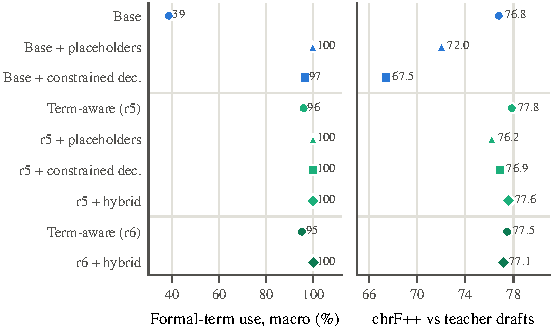
\includegraphics[width=\columnwidth]{figures/fig_tradeoff.pdf}
\caption{Inference-time enforcement: macro compliance and chrF++ against the teacher's translations, averaged over the four languages.}
\label{fig:tradeoff}
\end{figure}

\begin{table}[t]
\caption{Enforcement modes, mean over four languages. Det.\ = share of Maithili case endings after glossary terms written as a separate word.}
\label{tab:modes}
\centering
\footnotesize
\setlength{\tabcolsep}{4pt}
\begin{tabular}{@{}lrrrr@{}}
\toprule
System & Macro & chrF++ & BLEU & Det.\ (\%) \\
\midrule
Base & 38.5 & 76.8 & 61.6 & 1.4 \\
\quad + placeholders & 99.8 & 72.0 & 55.9 & 94.0 \\
\quad + constrained decoding & 96.7 & 67.5 & 33.9 & 4.7 \\
Term-aware r5 & 95.9 & 77.9 & 64.5 & 19.6 \\
\quad + placeholders & 99.9 & 76.2 & 61.8 & 97.4 \\
\quad + constrained decoding & 100.0 & 76.9 & 62.8 & 19.8 \\
\quad + hybrid & 100.0 & 77.6 & 64.2 & 0.0 \\
Term-aware r6 & 95.1 & 77.5 & 63.6 & 1.1 \\
\quad + hybrid & 100.0 & 77.1 & 63.3 & 0.0 \\
\bottomrule
\end{tabular}
\end{table}

\subsection{General-Domain Quality and Forgetting}
Fig.~\ref{fig:in22} reports the base model on IN22-Gen for all 22 scheduled languages, from 30.6 chrF++ (Kashmiri) to 66.2 (Urdu). Table~\ref{tab:forget} compares the adapted models on the four domain languages. All adapters stay within 0.5 chrF++ of the base model, and r6 within 0.41, so domain adaptation with LoRA did not cause measurable forgetting.

\begin{figure}[t]
\centering
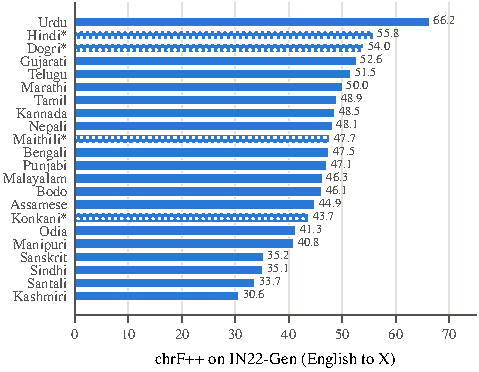
\includegraphics[width=\columnwidth]{figures/fig_in22.pdf}
\caption{Base model (dist-200M) on IN22-Gen, English to 22 languages (chrF++). Hatched bars and asterisks mark the four languages studied here.}
\label{fig:in22}
\end{figure}

\begin{table}[t]
\caption{Forgetting check on IN22-Gen (chrF++, human references).}
\label{tab:forget}
\centering
\footnotesize
\begin{tabular}{@{}lrrrr@{}}
\toprule
 & Hindi & Konkani & Maithili & Dogri \\
\midrule
Base & 55.77 & 43.71 & 47.68 & 54.02 \\
Distilled, raw drafts & 55.45 & 43.48 & 47.66 & 54.49 \\
Term-aware r5 & 55.31 & 43.51 & 47.47 & 54.15 \\
Term-aware r6 & 55.36 & 43.46 & 47.70 & 54.22 \\
\bottomrule
\end{tabular}
\end{table}

\subsection{Seeds, Joint Training and Morphology}
\emph{Seed variance.} Retraining r6 with a second seed changes chrF++ by 0.04 (Hindi), 0.98 (Konkani), 0.33 (Maithili) and 0.02 (Dogri), and pooled compliance by at most 3.6 points (Konkani). Differences below about one chrF++ point between single runs are therefore within training noise; this covers all differences between r5 and r6. Fig.~\ref{fig:dev} shows the dev curves. Dev scores of the raw-draft model are higher because its dev references are the same kind of raw drafts it imitates.

\begin{figure}[t]
\centering
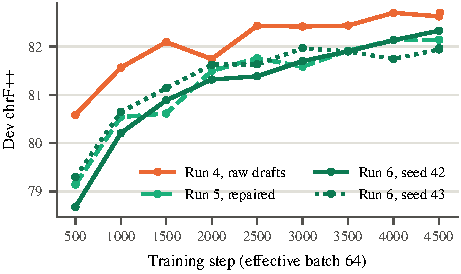
\includegraphics[width=\columnwidth]{figures/fig_dev_curves.pdf}
\caption{Dev chrF++ during training. Run 4 is scored against raw teacher drafts, runs 5 and 6 against repaired drafts.}
\label{fig:dev}
\end{figure}

\emph{Joint versus single-language training.} A Hindi-only adapter trained on the same Hindi data (24,009 pairs, 25 minutes) reaches 83.94 chrF++ and 97.9\% pooled compliance on the Hindi test set, against 83.83 and 98.6\% for the joint model. One joint adapter therefore serves four languages without a cost for Hindi.

\emph{Case endings.} Table~\ref{tab:case} shows that the r5 model learned the detached endings present in its training data, and that the rule-based correction of the data removed them in r6 for both seeds.

\begin{table}[t]
\caption{Case endings after glossary terms written as a separate word (detached / all occurrences).}
\label{tab:case}
\centering
\footnotesize
\begin{tabular}{@{}lrr@{}}
\toprule
System & Maithili & Konkani \\
\midrule
Base & 1 / 70 (1.4\%) & 0 / 12 (0\%) \\
Term-aware r5 & 18 / 92 (19.6\%) & 14 / 27 (51.9\%) \\
Term-aware r6, seed 42 & 1 / 93 (1.1\%) & 0 / 31 (0\%) \\
Term-aware r6, seed 43 & 0 / 97 (0\%) & 0 / 20 (0\%) \\
\bottomrule
\end{tabular}
\end{table}

% ============================================================================
\section{Discussion}

\emph{Why the teacher's terminology survives distillation.} The student learns to reproduce the teacher's output token by token, and a term rendered the same way in thousands of training sentences is among the easiest patterns to learn. Plain distillation even lowered compliance for Konkani, where the teacher uses loanwords more often than the base student. A larger teacher does not help either: the 1B model is never more than 1.5 points above the 200M base model on compliance. The terminology has to be corrected in the data.

\emph{Why repair the data instead of the output.} Enforcing terms at inference time works on any model, but it either damages the sentence (constrained decoding) or blocks morphology (placeholders), and it slows decoding. A model trained on repaired data produces the formal terms with normal fluency and inflects them, and the hybrid fallback is then needed for only 1.5\% of test sentences. The remaining misses concentrate on a few terms, such as \emph{circuit breaker} in Konkani (67\% compliance) and \emph{electric shock} in Hindi and Dogri.

\emph{Deployment.} We expose the models through a REST service that routes electrician content in the four languages to the r6 adapter with the hybrid fallback, and other languages to the base model. On a laptop CPU it needs about 0.9 s per sentence, or 0.33 s per sentence in batches of four, which is enough for on-demand localization of course pages.

% ============================================================================
\section{Limitations and Ethical Considerations}
\label{sec:limitations}

\emph{References.} The domain test references are unedited teacher translations, so we have no human-judged domain quality; chrF++ and BLEU on this set measure agreement with the teacher. Post-editing the test sets and a human evaluation by trainees and instructors are needed before any claim about translation quality.

\emph{Glossary.} The formal glossary was curated by the authors from NCERT and CSTT usage for Hindi and by analogy for the other three languages, without review by native-speaker instructors. Compliance measures adherence to this glossary, not correctness of the glossary. The glossary also has only 32 terms: related phrases outside it, such as \emph{earth connection}, are still sometimes rendered as \dev{पृथ्वी}, and hyphenated spellings such as \emph{three-phase} were not matched by our term detector and kept \dev{चरण}.

\emph{Register.} Formal terms may be less familiar to trainees than loanwords. Our method applies to either register; which one serves trainees best is an educational question that we did not test.

\emph{Scope and data rights.} We study one trade, four languages, a 200-sentence test set dominated by one term, and two training seeds, with machine-generated training targets. Some source books are marked as not for republication, so we release code, the glossary and the adapters but not the extracted text.

% ============================================================================
\section{Conclusion}

A strong multilingual teacher gives a student its fluency and also its terminology, including systematic wrong-sense terms. For electrician training content in Hindi, Konkani, Maithili and Dogri, repairing the teacher's translations with a formal glossary before distillation raised macro term compliance from 28--51\% to 90--99.6\% without affecting general-domain quality, and a hybrid fallback closed the remaining gap at a mean cost of 0.3 chrF++ points. Future work includes post-edited references and human evaluation, a reviewed glossary covering multi-word and hyphenated variants, other trades, and more languages, including Dravidian languages where case marking interacts more strongly with placeholder insertion.

\section*{Data and Code Availability}
Code, the glossary, model adapters and result files are available from the authors. The extracted sentences are not redistributed because of the licence of the source books.

\bibliographystyle{IEEEtran}
\bibliography{references}

\end{document}
